\documentclass[a4paper,12pt]{article}

% ==================================================
% PACKAGES
% ==================================================
\usepackage[authoryear,round]{natbib}
\usepackage{graphicx}
\usepackage{svg}
\usepackage{subcaption}
\usepackage{amsmath,amssymb}
\usepackage{iftex}
\ifPDFTeX
    \usepackage[utf8]{inputenc}
    \usepackage[T5]{fontenc}
\else
    \usepackage{fontspec}
    \setmainfont{Times New Roman}
\fi
\usepackage{geometry}
\usepackage{setspace}
\providecommand{\onehalfspacing}{\linespread{1.25}\selectfont}
\usepackage{float}
\usepackage{algorithm}
\usepackage{algpseudocode}
\usepackage{mdframed}
\usepackage{tikz}
\usepackage{enumitem}
\usepackage{xcolor}
\usepackage{colortbl}
\usepackage{placeins}
\usepackage{booktabs}
\usepackage{longtable}[=2020-01-02]
% Tương thích API footnote của longtable rollback với Hyperref hiện hành.
\makeatletter
\long\def\LT@p@ftntext#1{%
    \edef\@tempa{%
        \the\LT@p@ftn
        \noexpand\footnotetext[\the\c@footnote]%
    }%
    \global\LT@p@ftn\expandafter{\@tempa{#1}}%
}
\makeatother
\usepackage{array}
\usepackage{fancyhdr}
\usepackage[protrusion=false]{microtype}
\usepackage{tabularx}
\usepackage{multirow}
\usepackage[most]{tcolorbox}
\usepackage{listings}
% Hyperref được nạp sau các package tạo float/longtable để patch anchor đúng cách.
\usepackage[hypertexnames=false]{hyperref}

\usetikzlibrary{
    arrows.meta,
    positioning,
    shapes.geometric,
    shapes.misc,
    calc,
    fit
}

% ==================================================
% PAGE SETTINGS
% ==================================================
\geometry{
    top=1.7cm,
    bottom=1.7cm,
    left=2cm,
    right=2cm
}

\onehalfspacing
\setlength{\parindent}{0pt}

% ==================================================
% COLORS
% ==================================================
\definecolor{VinBlue}{RGB}{0,56,101}
\definecolor{VinRed}{RGB}{194,31,48}
\definecolor{VinGold}{RGB}{190,145,50}
\definecolor{LightGold}{RGB}{232,218,180}
\definecolor{MondBlue}{HTML}{173B57}
\definecolor{MondTeal}{HTML}{087E8B}
\definecolor{MondGold}{HTML}{E2A72E}
\definecolor{MondLight}{HTML}{F2F7F8}
\definecolor{MondRed}{HTML}{B54747}
\definecolor{MondGray}{HTML}{5B6770}
\definecolor{mondaiyblue}{HTML}{174B63}
\definecolor{mondaiyteal}{HTML}{167B7F}
\definecolor{mondaiylight}{HTML}{EEF5F4}
\definecolor{mondaiywarn}{HTML}{8A4B08}
\definecolor{codebg}{HTML}{F5F7F8}

\newcolumntype{Y}{>{\raggedright\arraybackslash}X}
\newcolumntype{P}[1]{>{\raggedright\arraybackslash}p{#1}}
\newtcolorbox{keybox}[1][]{
    colback=MondLight,
    colframe=MondTeal,
    boxrule=0.8pt,
    arc=2mm,
    title=#1,
    fonttitle=\bfseries
}
\newtcolorbox{warningbox}[1][]{
    colback=red!3,
    colframe=MondRed,
    boxrule=0.8pt,
    arc=2mm,
    title=#1,
    fonttitle=\bfseries
}
\newcommand{\assumption}{\textsuperscript{\color{MondGold}\bfseries [A]}}
\newcommand{\sourcefact}{\textsuperscript{\color{MondTeal}\bfseries [S]}}
\providecommand{\websrc}[2]{\footnote{\href{#1}{#2}.}}
\providecommand{\good}{\textbf{Có}}
\providecommand{\statuspartial}{\textbf{Một phần}}
\providecommand{\noevidence}{\textbf{Chưa thấy công bố}}
\newcommand{\code}[1]{\nolinkurl{#1}}
\newcommand{\implemented}{\textcolor{mondaiyteal}{\textbf{Đã triển khai trong mã nguồn}}}
% Evidence-status tags describe provenance, not quality.
\newcommand{\observed}{\texttt{OBSERVED\_STATIC\_DATA}}
\newcommand{\synthetic}{\texttt{SYNTHETIC\_BEHAVIOR}}
\newcommand{\modelestimate}{\texttt{MODEL\_ESTIMATE}}
\newcommand{\scenario}{\texttt{ASSUMPTION\_SCENARIO}}
\newcommand{\measured}{\texttt{EXPERIMENTALLY\_MEASURED}}
\newcommand{\warningnote}[1]{%
    \begin{quote}
        \color{mondaiywarn}\textbf{Lưu ý vận hành.} #1
    \end{quote}
}
\lstset{
    basicstyle=\ttfamily\small,
    backgroundcolor=\color{codebg},
    frame=single,
    breaklines=true
}
\lstdefinelanguage{json}{
    basicstyle=\ttfamily\small,
    string=[s]{"}{"},
    stringstyle=\color{VinBlue},
    comment=[l]{//},
    commentstyle=\color{MondGray},
    morecomment=[s]{/*}{*/},
    showstringspaces=false,
    breaklines=true
}

% ==================================================
% HYPERLINK SETTINGS
% ==================================================
\hypersetup{
    colorlinks=true,
    linkcolor=VinBlue,
    citecolor=VinBlue,
    urlcolor=VinBlue
}

\begin{document}
\setlength{\emergencystretch}{3em}
\raggedbottom
\sloppy
% Các bảng kỹ thuật có nhiều chuỗi định danh dài; cho phép TeX dùng khoảng co giãn
% khẩn cấp mà không phát sinh cảnh báo hộp giả trong log.
\hbadness=10000
\vbadness=10000
\hfuzz=400pt
\vfuzz=400pt
\AddToHook{para/begin}{\hbadness=10000\hfuzz=\maxdimen}
\renewcommand*{\theHtable}{\arabic{table}.\arabic{page}}
\hypersetup{pageanchor=false}

% ==================================================
% COVER PAGE
% ==================================================
\begin{titlepage}
\thispagestyle{empty}

% Decorative page border
\begin{tikzpicture}[remember picture,overlay]
    % Outer border
    \draw[
        VinBlue,
        line width=2pt
    ]
    ($(current page.north west)+(0.75cm,-0.75cm)$)
    rectangle
    ($(current page.south east)+(-0.75cm,0.75cm)$);

    % Inner border
    \draw[
        VinGold,
        line width=0.8pt
    ]
    ($(current page.north west)+(0.92cm,-0.92cm)$)
    rectangle
    ($(current page.south east)+(-0.92cm,0.92cm)$);

    % Decorative corner accents
    \draw[
        VinGold,
        line width=2pt
    ]
    ($(current page.north west)+(0.75cm,-1.55cm)$)
    to
    ($(current page.north west)+(0.75cm,-0.75cm)$)
    to
    ($(current page.north west)+(1.55cm,-0.75cm)$);

    \draw[
        VinGold,
        line width=2pt
    ]
    ($(current page.north east)+(-1.55cm,-0.75cm)$)
    to
    ($(current page.north east)+(-0.75cm,-0.75cm)$)
    to
    ($(current page.north east)+(-0.75cm,-1.55cm)$);

    \draw[
        VinGold,
        line width=2pt
    ]
    ($(current page.south west)+(0.75cm,1.55cm)$)
    to
    ($(current page.south west)+(0.75cm,0.75cm)$)
    to
    ($(current page.south west)+(1.55cm,0.75cm)$);

    \draw[
        VinGold,
        line width=2pt
    ]
    ($(current page.south east)+(-1.55cm,0.75cm)$)
    to
    ($(current page.south east)+(-0.75cm,0.75cm)$)
    to
    ($(current page.south east)+(-0.75cm,1.55cm)$);
\end{tikzpicture}

\begin{center}

% Organization
{\fontsize{16}{20}\selectfont
 \color{VinBlue}
 \textbf{HANOI UNIVERSITY OF SCIENCE AND TECHNOLOGY}
}

\vspace{0.15cm}

{\fontsize{16}{20}\selectfont
 \textbf{School of Information and Communication Technology}
}

\vspace{0.25cm}

% Line under program name

\begin{tikzpicture}
    \draw[VinGold,line width=1.2pt] (0,0) to (13.5,0);
    \fill[VinRed] (6.55,-0.06) rectangle (6.95,0.06);
\end{tikzpicture}

\vspace{0.35cm}

% Organization logos
\begin{minipage}[c][4.2cm][c]{0.46\textwidth}
    \centering
    
\includegraphics[
        height=3.8cm,
        keepaspectratio
    ]{figure/HUST.png}
\end{minipage}
\hfill
\begin{minipage}[c][4.2cm][c]{0.46\textwidth}
    \centering
    
\includegraphics[
        width=6.2cm,
        trim=46 180 44 177,
        clip
    ]{figure/soict.png}
\end{minipage}

\vspace{0.55cm}

% Project heading
{\fontsize{23}{28}\selectfont
 \color{VinBlue}
 \textbf{PROJECT REPORT}
}

\vspace{0.15cm}

{\color{VinGold}\rule{7cm}{1pt}}

\vspace{0.3cm}

{\fontsize{19}{23}\selectfont
 \color{VinBlue}
 \textbf{Customer Churn Prediction and Segmentation for a Digital Bank}\\[0.04cm]
}

\vspace{0.5cm}

\vfill

\begin{minipage}{0.80\textwidth}
    \renewcommand{\arraystretch}{1.15}
    \begin{tabularx}{\linewidth}{@{}>{\bfseries}l@{\hspace{0.6cm}}X@{}}
        Course: & Intro To Business Analyst \\
        Class ID: & 175884 \\
        Supervisor: & Ph.D Bui Quoc Trung \\
    \end{tabularx}
\end{minipage}

\vfill

\begin{minipage}{0.80\textwidth}
    \small
    \begin{tabularx}{\linewidth}{@{}>{\bfseries}X@{\hspace{0.7cm}}r@{}}
        \toprule
        Member & Student ID \\
        \midrule
        Hoang Trong Tan & 202416751 \\
        Vu Thuong Tin & 20230091 \\
        Tran Quang Huy & 202416706 \\
        Nguyen Le Duc Anh & 20235472 \\
        Nguyen Duc Dung & 202416681 \\
        \bottomrule
    \end{tabularx}
\end{minipage}

\vspace{0.55cm}

% Footer
{\color{VinGold}\rule{5cm}{0.8pt}}

\vspace{0.15cm}

{\large\color{VinBlue}\textbf{Ha Noi, 2026}}

\end{center}
\end{titlepage}
\clearpage

% ==================================================
% HEADER AND FOOTER FOR THE FOLLOWING PAGES
% ==================================================
\pagenumbering{arabic}
\hypersetup{pageanchor=true}
\pagestyle{fancy}
\setlength{\headheight}{15pt}
\fancyhf{}
\fancyhead[L]{\color{VinBlue}\small\textbf{Beyond the Haze}}
\fancyhead[R]{\color{VinBlue}\small\textbf{Project Charter}}
\fancyfoot[C]{\thepage}
\renewcommand{\headrulewidth}{0.6pt}
\renewcommand{\footrulewidth}{0pt}

\tableofcontents
\clearpage
\listoffigures
\clearpage
\listoftables
\clearpage
\section*{List of abbreviations}
\begin{longtable}{p{0.20\textwidth}p{0.70\textwidth}}
A/B & Randomized comparison of a treatment arm against a control or alternative arm\\
API & Application Programming Interface\\
ARI & Adjusted Rand Index\\
CI & Confidence interval\\
CRM & Customer Relationship Management\\
K-Means & K-means clustering algorithm\\
KPI & Key Performance Indicator\\
MDE & Minimum Detectable Effect\\
MLOps & Model deployment, monitoring and governance practices\\
OOD & Out-of-distribution\\
PCA & Principal Component Analysis\\
PR-AUC & Area under the precision--recall curve\\
ROC-AUC & Area under the receiver operating characteristic curve\\
SLA & Service Level Agreement\\
\end{longtable}
\clearpage

% ==================================================
% REPORT BODY
% All substantive report text is intentionally kept in this file.
% ==================================================
\section{Introduction}

\paragraph*{The churn problem.}
Customer churn is the progressive loss of a banking relationship: a customer reduces the share of payments, deposits, borrowing, or service interactions conducted with one provider and eventually moves part or all of that relationship elsewhere. It is more consequential than closing one card or leaving one balance unchanged. Banks lose future transaction activity, product usage, fee and margin opportunities, and the accumulated value of a relationship that took time and money to acquire. The operational challenge is to recognise weakening relationships early enough to respond with a relevant service, product, or communication before the customer has completed the move.

\paragraph*{Why the problem is becoming more urgent.}
Financial access and digital connectivity now operate at global scale. The World Bank's \textit{Global Findex 2025}, based on nationally representative surveys of about 148,000 adults in 141 economies, reports that 79\% of adults worldwide had a financial account in 2024, up from 51\% in 2011 and 74\% in 2021 \citep{worldbank2025,worldbank2025press}. Account ownership reached 75\% in low- and middle-income economies, while 86\% of adults globally owned a mobile phone \citep{worldbank2025}. This expansion brings banking into the customer's everyday digital environment, where comparison, account opening, payment choice, and customer-service expectations are immediate. In Baringa's 2025 survey of 4,000 retail-banking customers in the United Kingdom and the United States, more than one third had switched provider in the preceding five years, and 62\% said they would switch for a better digital experience \citep{baringa2025}. Retention has therefore become a continuous operating decision rather than a periodic marketing exercise.

\paragraph*{The scale of customer exit.}
Research in financial services shows why banks need to treat attrition as a portfolio problem. Van den Poel and Larivi\`ere analysed a random sample of 47,157 customers from a European financial-services company using longitudinal data; 47\% experienced the churn event during the observation period \citep{vandenpoelLariviere2004}. Their study combines relationship history, customer behaviour, demographics, and macro-environmental conditions, illustrating the breadth of information required to understand attrition over time. Evidence from Asia points to the same need for prioritisation. Ahn, Kim, and Lee examined complete trading records and customer profiles for 458,098 retail customers at a Korean brokerage house; in their study, the density of inactive customers in the top 10\% most-likely-to-churn group was five to six times the unconditional attrition ratio \citep{ahnKimLee2020}. The commercial task is not to contact every customer. It is to direct finite service, CRM, and product capacity toward the relationships where timely action is most likely to matter.

\paragraph*{Why customers switch banks.}
Bank switching reflects concrete failures and trade-offs that customers encounter. In a study of 694 retail-banking customers in Australia and New Zealand, Colgate and Hedge identified three principal problem areas preceding switching: service failures, pricing problems, and denied services. Pricing problems had the strongest effect on switching, whereas service failures generated more complaints before exit \citep{colgateHedge2001}. The wider service-switching literature reaches a similarly specific conclusion. Keaveney's critical-incident study of more than 500 service customers identified more than 800 switching behaviours and grouped them into eight categories, including price, inconvenience, core-service failure, failed service encounters, inadequate responses to failure, competition, ethical problems, and involuntary switching \citep{keaveney1995}. For a bank, these findings turn churn from an abstract percentage into a set of customer journeys that can be observed, assigned, and improved: failed payments, unclear charges, long waits, poor recovery after an error, and digital tasks that do not work as expected.

\paragraph*{What predictive analytics can change.}
Churn analytics gives a bank a disciplined way to concentrate attention. Transaction recency and frequency, product use, digital engagement, service cases, and relationship tenure can identify groups whose behaviour differs materially from the broader portfolio. A risk score helps order a review queue; behavioural segmentation clarifies what type of engagement the customer has; eligibility rules protect customers who should not be contacted; and value rules set a cost boundary for the intervention. These components create a decision process rather than a list of names. Each action should specify its customer trigger, channel, owner, cost, expected mechanism, and measurable outcome. Service recovery, for example, requires a different workflow from an onboarding intervention or an explanation of product fees.

\paragraph*{The decision question.}
The central question is therefore not simply \emph{who is likely to churn?} It is \emph{which customers should the bank contact, why, through which channel, at what cost, and how will the bank know whether the action worked?} Answering it requires the integration of churn prediction, behavioural segmentation, customer eligibility, operational capacity, and experimental measurement. The objective of this report is to frame customer retention as a governed decision system: one that directs attention toward the right relationship, proposes a specific next step, and measures whether that step improves customer outcomes and bank performance.

\section{Problem Statement}

Bank X is the pseudonymous digital retail bank used for this case. Its customer portfolio comprises 10,000 unique records with credit score, country, gender, age, tenure, balance, product count, card ownership, active-member status, estimated salary, and a relationship-exit label \citep{topreKaggle}. The bank operates across France, Germany, and Spain: France represents 5,014 customers (50.14\%), Germany 2,509 (25.09\%), and Spain 2,477 (24.77\%). The portfolio is primarily a one- or two-product base, with 5,084 customers holding one product and 4,590 holding two. At the same time, 4,849 customers are recorded as inactive members. These are the operating conditions under which Bank X must protect and deepen customer relationships.

The immediate business problem is the size and concentration of customer exit. Bank X records 2,037 exits, equivalent to a churn rate of 20.37\% across the portfolio \observed. Churn is not evenly distributed. Germany has 814 exits among 2,509 customers, a rate of 32.44\%, while France and Spain record 16.15\% and 16.67\%, respectively. The inactive-member cohort has a churn rate of 26.85\% (1,302 of 4,849 customers), compared with 14.27\% for active members (735 of 5,151). Product depth shows a similarly pronounced difference: 27.71\% of one-product customers exited (1,409 of 5,084), against 7.58\% of two-product customers (348 of 4,590). For Bank X, the challenge is therefore not simply to reduce an average churn rate; it is to address materially different retention pressures across markets, relationship depth, and customer activity.

This pattern creates a management problem. A single retention message cannot address a customer whose relationship has weakened, a customer facing an unresolved service issue, and a customer who needs clearer product value. Nor can CRM allocate capacity solely on the basis of a portfolio average. Bank X needs a common decision process that determines which customers merit attention, what type of intervention fits the relationship, which channel and team should deliver it, and how much the bank should be willing to spend. That process must also prevent unsuitable contact, including promotional outreach to customers who require service recovery or who should be suppressed from contact.

The business requirement is therefore a customer-intelligence and retention-decision system for Bank X. It must translate the portfolio into actionable customer groups, rank eligible customers by retention priority, and connect each priority to a specific intervention, owner, channel, and cost boundary. Executives need a clear view of where churn is concentrated and where investment should be directed. CRM needs a governed contact queue. Product and Operations need evidence on the journeys most likely to require improvement. Finance needs a transparent basis for evaluating the cost of intervention against the value of retaining a customer. The case asks Bank X to decide where to intervene first, how to intervene, and how to demonstrate that the chosen action improves retention.

\section{Background}

\subsection{Retail banking}

Retail banking is a relationship business. Customers use banks to receive income, hold deposits, pay merchants and bills, transfer money, borrow, manage cards, and obtain assistance when a transaction or product does not work as expected. Over time, a relationship normally progresses from onboarding and account funding to regular use, product deepening, and a position as the customer's primary financial provider. Digital banking compresses this journey into a series of app, web, card, payment, and service interactions. Each interaction can strengthen convenience and trust or encourage the customer to divide activity across competing providers.

The relationship is broader than any single account. A customer may close a card while retaining deposits, maintain an open account while moving regular payments elsewhere, or hold a balance without treating the bank as a primary provider. Customer churn refers to the loss of the overall relationship; product attrition refers to the loss of one product; dormancy refers to the absence of qualifying activity over a defined period; and balance flight refers to a sustained reduction in deposits. These are different business events. They require different measures, different customer journeys, and different responses from Product, CRM, and Operations.

\subsection{Customer churn}

Customer exit is usually the outcome of repeated decisions rather than a single event. A customer may begin by reducing transaction frequency, using another bank for salary receipt or payments, allowing an account to become inactive, or seeking help after a failed transaction. The final act of closing an account may occur much later. Longitudinal evidence from a European financial-services company shows why time matters: Van den Poel and Larivi\`ere modelled attrition for 47,157 customers using relationship history, behavioural information, demographics, and macro-environmental conditions, and identified critical periods early in the customer relationship \citep{vandenpoelLariviere2004}.

The drivers are concrete. In a study of 694 retail-banking customers in Australia and New Zealand, Colgate and Hedge found that switching followed service failures, pricing problems, and denied services; pricing problems had the largest effect on switching, while service failures generated more complaints before exit \citep{colgateHedge2001}. Keaveney's study of more than 500 service customers identified over 800 critical switching behaviours, grouped into pricing, inconvenience, core-service failures, failed service encounters, inadequate responses to failure, competition, ethical problems, and involuntary switching \citep{keaveney1995}. For banks, these categories translate into recognisable customer experiences: an unexplained charge, an unsuccessful payment, a difficult digital task, a long wait for support, or poor recovery after an error.

\subsection{Retention economics}

Churn affects the economics of a bank in three ways. First, it removes future contribution from deposits, payments, lending, and related products. Second, it increases the pressure to acquire and onboard replacement customers. Third, it can reveal a product or service weakness that affects many customers before it appears in aggregated financial reporting. The commercial case for retention is therefore not simply to keep an account open. It is to preserve a profitable, trusted, and active relationship while directing service resources to the points where they create the greatest value.

The appropriate economic measure is incremental contribution. A retention programme creates value when the additional contribution retained because of the intervention exceeds the cost of contact, incentive, service delivery, and measurement. Customer balance, transaction volume, and estimated salary are inputs to understanding a relationship; they are not measures of profit. This distinction matters because a campaign aimed at a high-balance customer may still destroy value if the intervention is expensive, poorly targeted, or inappropriate for the customer's need.

\subsection{Retention decisions}

Churn prediction and retention management answer different questions. A propensity model ranks customers by their likelihood of an observed exit. Behavioural segmentation groups customers with similar usage patterns and service needs. A value tier sets the financial importance of the relationship. Eligibility rules determine whether a customer may be contacted at all. Combining these components enables a bank to move from a generic risk list to a decision: whether to provide service recovery, onboarding support, digital assistance, a product review, or no contact.

The quality of that decision depends on measurement. A high propensity score identifies a relationship that deserves attention; it does not determine whether a specific intervention will change the outcome. Banks therefore need an eligible customer population, a defined treatment, an appropriate comparison group, and recorded outcomes such as retention, customer activity, complaint, opt-out, and cost. This turns churn management into a business discipline: identify the relationship at risk, choose an action that addresses the relevant customer need, and measure the commercial and customer impact of that action.

\section{Data}

\subsection{Data overview}

The analysis uses the course-specified Kaggle \emph{Bank Customer Churn Dataset}, published by Gaurav Topre \citep{topreKaggle}. It is a static, customer-level retail-banking dataset: each row represents one customer relationship, and the relationship-exit outcome is recorded in the \texttt{Exited}/\texttt{churn} label. The source supports portfolio profiling, historical churn analysis, and supervised-model development; it provides the starting point for the Bank X case described in the preceding section.

The preprocessing run reads and retains all 10,000 source rows. It finds no duplicate customer IDs, no missing values in the retained fields, and no rows requiring deletion or imputation. The resulting analysis base separates the customer attributes from the churn label, preventing the outcome from entering segmentation or feature-generation inputs. The portfolio's historical churn prevalence is 20.37\% (2,037 of 10,000 customers). Appendix~\ref{app:data-dictionary} provides the complete field-level dictionary, including type, business meaning, and analytical role.

\subsection{Data provenance and preparation}

The preparation pipeline is versioned as \texttt{kaggle-static-preprocess-v1}. Its quality manifest records the source-file checksum, the row-level audit, the target-separation rule, and hashes for the resulting customer and label tables. The raw-file SHA-256 is \texttt{90f6625c31bdfcb0cde3b94c4f3004e43795e382921d0a5be67c4bd490b38818}. The source label is retained as a historical relationship-exit outcome; it is not used to construct behavioural segments or generate the primary behavioural extension.

The source provides a cross-sectional customer profile rather than a transaction ledger. It contains no timestamps for observation, scoring, or outcome windows, and it contains no campaign assignment, contact preference, service-case, transaction, or realised contribution record. Those data requirements shape the synthetic behavioural design and the later retention-measurement plan. The source currency for balance and estimated salary is unspecified, so both are treated as profile variables rather than contribution or customer-lifetime-value measures.

\begin{table}[H]
\centering
\caption{Static source contract and handling [\observed].}
\label{tab:static-contract}
\small
\begin{tabularx}{\textwidth}{P{0.27\textwidth}Y}
\toprule
\textbf{Element} & \textbf{Contract and limitation}\\
\midrule
Grain & One row per pseudonymous source customer; unique, nonblank identifier required.\\
Fields & Demographic/profile fields, product count, balance, estimated salary, active-member flag, and static historical churn label.\\
Quality outcome & 10,000 read; 10,000 retained; 0 duplicates; 0 retained nulls; 0 rows dropped.\\
Target boundary & \texttt{churn} is stored separately from model-ready customer attributes.\\
Time semantics & No observation date, event history, prediction point, or label window. A next-quarter claim is unsupported.\\
Sensitive/proxy fields & Gender and country are excluded from behavioural clustering and proposed treatment selection.\\
Financial semantics & Balance and estimated salary use unspecified source currency; neither is contribution or CLV.\\
\bottomrule
\end{tabularx}
\end{table}

\subsection{Synthetic behavioural data}

The static base has no transaction, app, channel, or service-case history. It cannot answer whether a customer was recently active, whether app use is declining, whether a payment failed, or whether an unresolved case should suppress an offer. To rehearse those analytical and engineering requirements, the project generates six monthly periods of labelled \synthetic{} data using a fixed seed. The generator receives only label-free static attributes and seeded random variation. It explicitly rejects an input table that contains \texttt{churn}, so the primary behavioural simulation is not label-conditioned.

The resulting tables model a minimal customer-event architecture: customer-month balance-flow scenarios, transaction-month channel and type facts, digital-month app activity and failed-payment scenarios, simulated service cases, a cutoff-safe feature snapshot, and a segment assignment. The generator verifies grains and basic plausibility: exactly six customer-month rows per customer, non-negative transaction counts and amounts, app-active days in 0--31, sessions no fewer than active days, valid case timelines, and a unique feature row per customer. A synthetic incoming-flow event is specifically not interpreted as an observed salary payment; a synthetic loan repayment is not evidence of actual loan ownership.

\begin{table}[H]
\centering
\caption{Canonical analytical tables and provenance [\observed{} + \synthetic].}
\label{tab:data-model}
\small
\begin{tabularx}{\textwidth}{P{0.28\textwidth}P{0.25\textwidth}Y}
\toprule
\textbf{Table} & \textbf{Grain} & \textbf{Purpose and source status}\\
\midrule
\texttt{customer\_base} & one customer & Static profile; \observed.\\
\texttt{customer\_snapshot} & customer $\times$ simulated month & Simulated inbound/outbound-flow scenario; \synthetic.\\
\texttt{transaction\_month} & customer $\times$ simulated month $\times$ channel/type & Simulated count and amount; \synthetic.\\
\texttt{digital\_month} & customer $\times$ simulated month & Simulated active days, sessions, feature, failed payment; \synthetic.\\
\texttt{service\_case} & simulated case & Simulated open/resolved lifecycle and category; \synthetic.\\
\texttt{feature\_snapshot} & customer $\times$ cutoff & Features computed using months at or before cutoff; \synthetic.\\
\texttt{segment\_assignment} & customer $\times$ segment version & Label-free behavioural grouping; \synthetic.\\
\texttt{risk\_prediction} & customer $\times$ model version & Planned only; no trained artifact exists yet.\\
\bottomrule
\end{tabularx}
\end{table}

The extension supports method development and interface testing, not discovery of actual customer motives. Its correlations are construction assumptions. Changing the seed changes simulated customers; it does not constitute external validation. Every display below marks whether its numbers originate in the static base, the simulation, a future model estimate, or a scenario.

\subsection{Analytical design}

The workflow deliberately separates descriptive analysis, segmentation, prediction, and treatment measurement. First, static fields support a source audit and historical cohort descriptions. Second, simulation produces event facts and cutoff-safe behavioural features. Third, clustering is fit without the churn label, IDs, gender, or country. Only after assignment is frozen is the historical static label joined for a descriptive cross-tab. Fourth, a later classification pipeline must use train-only transformations, untouched test data, calibration, subgroup diagnostics, and capacity-based threshold selection. Finally, treatment performance is measured by a future randomized pilot, not imputed from a churn score.

This sequence controls several common errors: target leakage into clustering, learning transformations from the holdout, confusing synthetic behaviour with observation, calling balance a value metric, and converting association into causal explanation. It also creates a practical audit trail: every table declares grain; each derived file has a version and source tag; and user-facing recommendations can cite the artifact that produced them.

\section{Customer analysis and behavioural segmentation}

\subsection{Analytical question and evidence status}

The completed customer-analysis module asks a narrow, decision-relevant question: \emph{within a six-month synthetic behavioural rehearsal, are there stable, operationally distinct usage patterns that justify different service and experiment hypotheses?} It does not ask which customers will certainly churn, which customer has a particular need, or which treatment will create retention. The answer is based on a V3 K-Means baseline fitted to all 10,000 simulated feature snapshots and then overlaid with the static historical label for description only.

Nine behaviour-only features enter the baseline: six-month transaction count and amount, app-active days, failed payments, simulated inbound flow and number of inflow months, cash-withdrawal share, an inflow trend ratio, and unresolved-case share. Positive skewed counts and amounts are transformed with \texttt{log1p}; the feature matrix is standardized before K-Means. The churn label is absent from the generator, feature construction, and cluster fitting. Segment IDs are then made interpretable by labelling the group with higher mean app-active days as \texttt{segment\_high\_digital}; this is a neutral behavioural description, not a value judgement.

The V3 baseline produces a silhouette value of 0.373. Across five full generator-plus-clustering runs with seeds 11, 23, 37, 53, and 71, the high-digital segment share lies between 52.46\% and 52.70\%; adjusted Rand index relative to seed 11 ranges from 0.875 to 0.885 for the other four runs. These diagnostics show that this particular simulated construction gives a repeatable two-group split. They do not prove that two true customer personas exist at a real bank. The current V3 artifact also lacks a documented comparison across adjacent $k$ values and alternative clustering algorithms; therefore $k=2$ is a transparent operational baseline, not a final scientific optimum. That gap must be closed before a production-like segmentation gate can pass.

\begin{figure}[H]
\centering
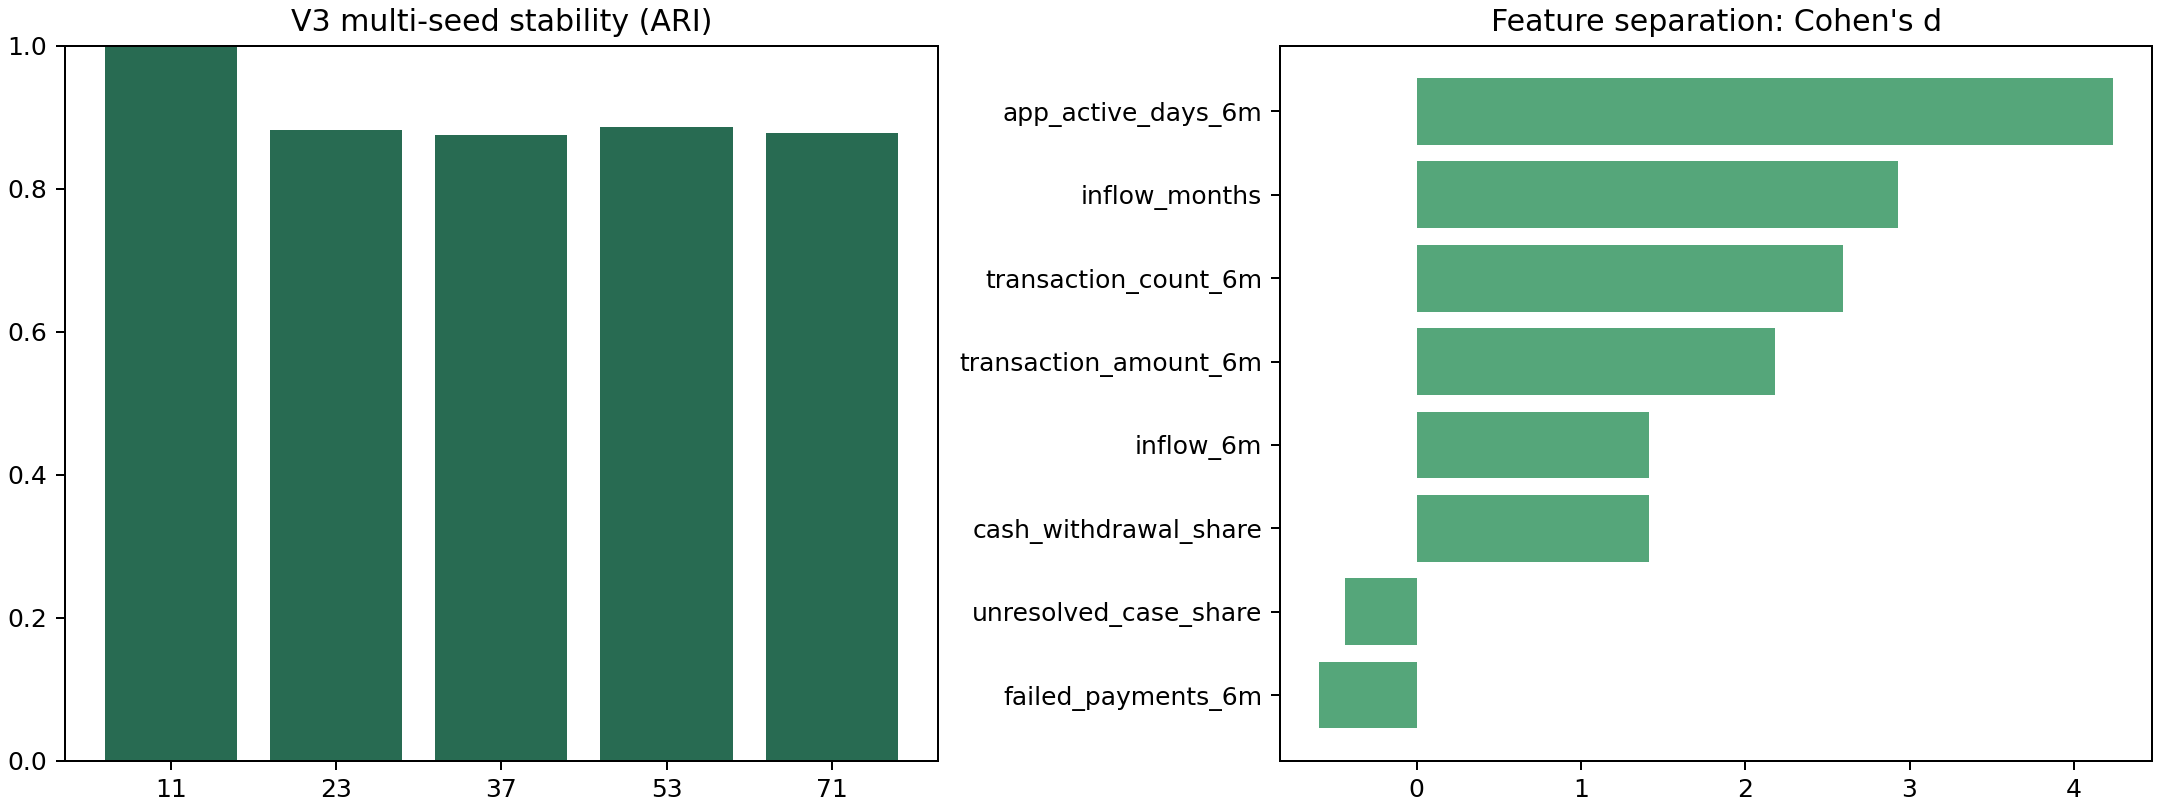
\includegraphics[width=0.95\textwidth]{figure/v3_stability_and_distinctiveness.png}
\caption{[\synthetic] V3 five-seed stability diagnostic and behaviour-feature separation. The chart assesses repeatability of the simulated pipeline, not validation of real bank personas.}
\label{fig:stability}
\end{figure}

\subsection{Portfolio-level result: two different behavioural patterns}

The two groups are operationally large and almost balanced. The high-digital-routine segment contains 5,285 customers (52.85\%); the lower-digital-relationship segment contains 4,715 (47.15\%). Table~\ref{tab:segment-profile} reports the cluster profiles. All rows except historical-label columns are derived from the synthetic extension. The strongest separation is app-active days: 67.17 versus 24.42 days over six simulated months (Cohen's $d=4.24$). The high-digital group also has more inflow months and more simulated transactions. The lower-digital group has more failed payments and a larger unresolved-case share.

Those differences support differentiated operational hypotheses. They do not establish customer satisfaction, financial distress, the reason for a failed payment, or the cause of churn. In particular, the cash-withdrawal-share result is an artefact of the present generator: it is identical at one-third in both groups while the reported standardized difference is distorted by negligible within-group variance. It should not be used in a segment narrative or treatment rule until the feature definition and diagnostic are corrected. Surfacing this anomaly is preferable to silently using an attractive but unstable feature.

\begin{table}[H]
\centering
\caption{V3 behavioural segment profile, six simulated months; historical label shown only as a post-fit overlay [\synthetic{} + \observed].}
\label{tab:segment-profile}
\small
\begin{tabularx}{\textwidth}{Y P{0.22\textwidth}P{0.22\textwidth}P{0.19\textwidth}}
\toprule
\textbf{Measure} & \textbf{High digital routine} & \textbf{Lower digital relationship} & \textbf{Evidence class}\\
\midrule
Customers, share & 5,285; 52.85\% & 4,715; 47.15\% & \synthetic{} assignment\\
App-active days, 6m (mean) & 67.17 & 24.42 & \synthetic{}; $d=4.24$\\
Inflow months, 6m (mean) & 4.83 & 1.35 & \synthetic{}; $d=2.93$\\
Transaction count, 6m (mean) & 41.71 & 26.35 & \synthetic{}; $d=2.60$\\
Transaction amount, 6m (mean) & 1,415.51 & 824.41 & \synthetic{}; source currency unspecified; $d=2.18$\\
Failed payments, 6m (mean) & 0.25 & 0.64 & \synthetic{}; $d=-0.59$\\
Unresolved-case share (mean) & 7.28\% & 20.91\% & \synthetic{}; $d=-0.44$\\
Static historical churn label & 751/5,285 = 14.21\% & 1,286/4,715 = 27.27\% & \observed{} post-fit cross-tab\\
95\% Wilson CI for label rate & 13.29\%--15.18\% & 26.02\%--28.56\% & \observed{} post-fit cross-tab\\
\bottomrule
\end{tabularx}
\end{table}

The observed-static cross-tab differs by 13.06 percentage points: the lower-digital group has a historical label rate about 1.92 times that of the high-digital group. This is a useful prioritisation signal for an exploratory pilot design, subject to the source limitations. It is not a forecast, an individual probability, or evidence that low app activity caused exit. The simulation itself is conditioned on static fields such as the recorded active-member flag, age, product count, and estimated salary; it therefore cannot be used to discover a causal engagement mechanism that has already been embedded in the generator.

\begin{figure}[H]
\centering
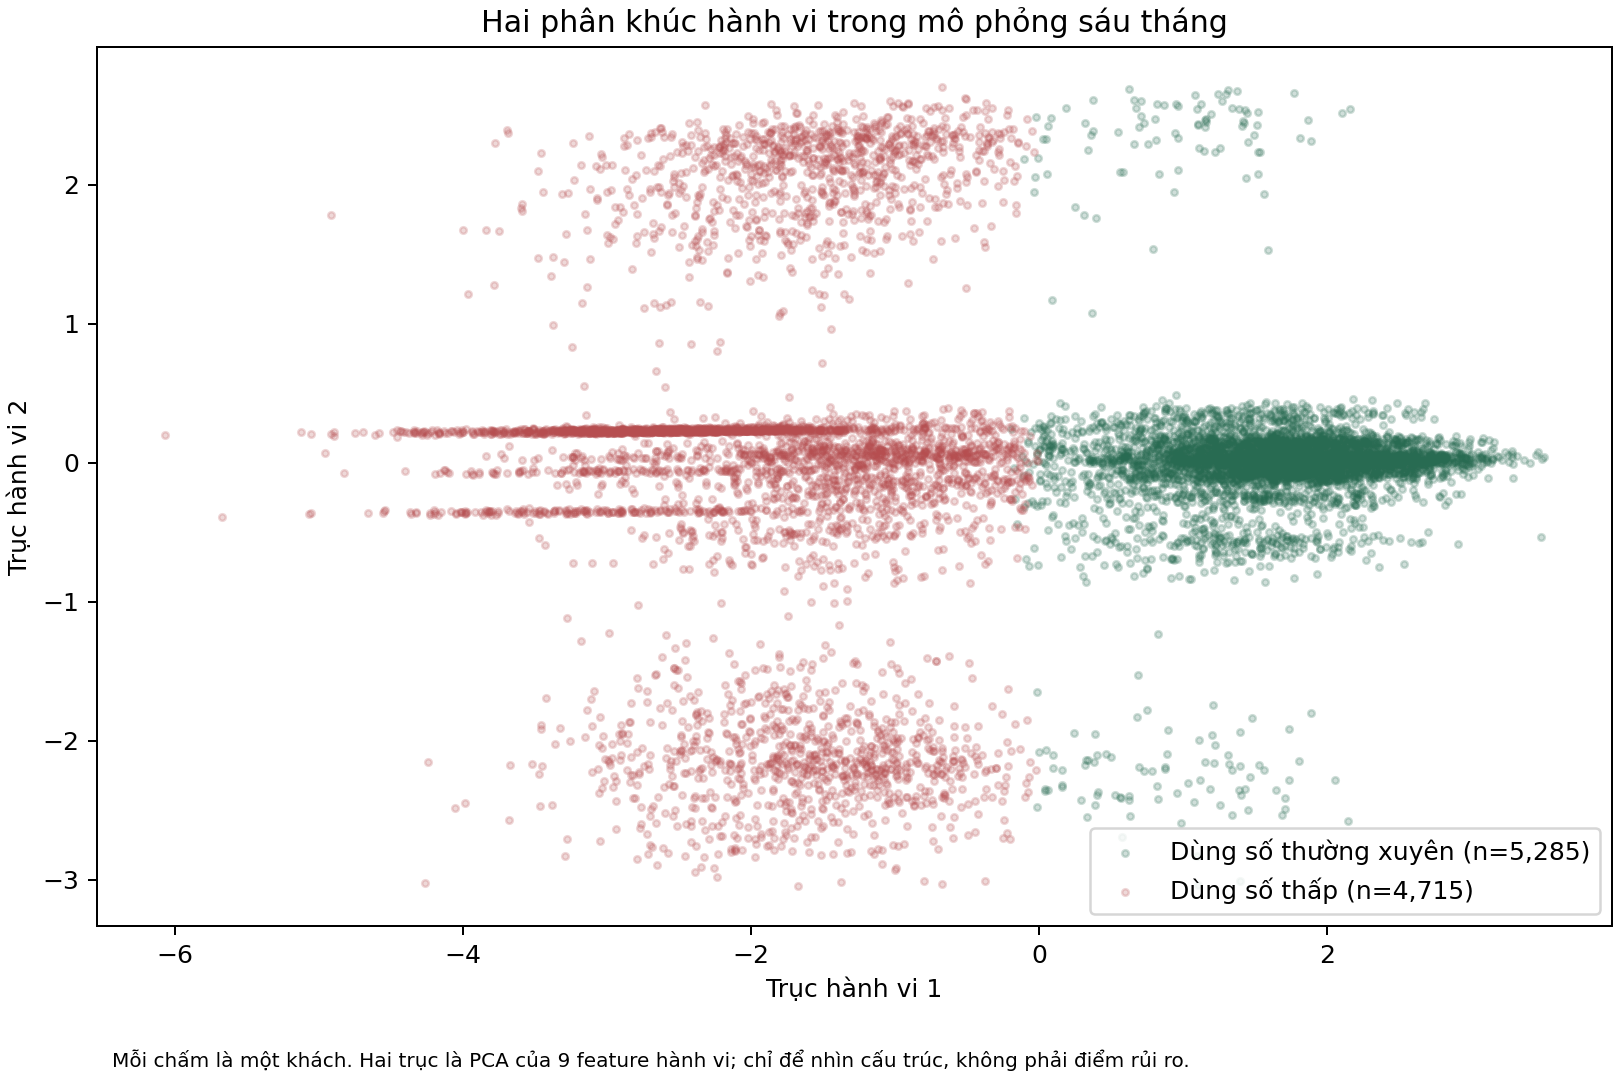
\includegraphics[width=0.82\textwidth]{figure/v3_cluster_map.png}
\caption{[\synthetic] Two V3 behavioural groups in a PCA projection of the simulated feature space. The projection is a visual summary only; it is neither a risk score nor a treatment recommendation.}
\label{fig:clusters}
\end{figure}

\subsection{Concrete persona dossiers: Linh and Minh}

To make the segment cards usable by CRM, Product, and Care, the project gives each behavioural pattern a synthetic persona handle. \textbf{Linh} and \textbf{Minh} are not customers, not representative individuals, and not customer records. Their names make the operating distinction memorable; every behavioural detail below remains a group-level \synthetic{} result, while the profile fields and historical label cross-tabs are \observed{}. Gender, recorded country, estimated salary, and balance are never used to choose a channel, offer, price, or eligibility.

\subsubsection{Persona A --- Linh: regular digital self-service relationship}

\textbf{Who Linh represents.} Linh represents 5,285 customers (52.85\% of the portfolio). In the static base, this group has mean age 39.6, mean credit score 653.2, 44.4\% recorded female, 97.0\% with the active-member flag, and a mean of 1.54 products. France is the recorded source category for 50.3\% of the group, Spain for 25.5\%, and Germany for 24.2\%. Median estimated salary is 100,240 and median balance is 95,984 in an unspecified source currency. These numbers describe the static extract only: they are not income, wealth, contribution, CLV, or evidence of a product need.

\textbf{What the simulated six months show.} Linh opens the app 67.17 days in six months, or about 11.2 days in a typical simulated month. Her group records 4.83 simulated inflow months and 41.71 transactions in six months. The main synthetic app activity is \texttt{transfers\_and\_bill\_pay} (26,472 customer-months); \texttt{balance\_and\_card\_controls} appears in another 4,308 customer-months. Failed payments average 0.25 per customer over six months and unresolved-case share is 7.28\%. This is a pattern of frequent digital self-service, not proof of satisfaction or loyalty.

\textbf{Why it matters.} The static historical label rate is lower than the other segment at 14.21\% (751/5,285), but the group is large. A poorly designed transfer, bill-payment, or card-control flow could inconvenience many customers before it emerges as a complaint. The operational hypothesis is therefore to protect routine completion rather than to send a blanket incentive.

\begin{table}[H]
\centering
\caption{Linh persona: evidence, hypothesis, and control [\synthetic{} + \observed{} + \scenario].}
\label{tab:linh-persona}
\small
\begin{tabularx}{\textwidth}{P{0.20\textwidth}Y}
\toprule
\textbf{Dimension} & \textbf{Operational interpretation}\\
\midrule
Strength & An established simulated self-service routine makes contextual help feasible.\\
Weakness & Friction in a frequently used task can damage the experience at scale.\\
Opportunity & Test a task-specific shortcut, clear processing status, and one-step escalation to Care.\\
Threat & Irrelevant sales outreach can create contact fatigue or distract from a system fault.\\
Need to test & Does reducing routine-task friction retain more customers than a transparent, opt-in explanation of existing fees and benefits?\\
Treatment comparison & Digital Concierge versus Value Review; neither arm may use an automatic incentive or default cross-sell.\\
Primary outcome & Incremental 90-day retention; leading indicators are task completion, failed-task-to-support rate, repeat support contact, opt-out, and complaint.\\
Falsification & No positive retention effect with a lower 95\% CI above zero, or guardrails worsen versus the comparator.\\
\bottomrule
\end{tabularx}
\end{table}

\subsubsection{Persona B --- Minh: thin digital relationship, recovery first}

\textbf{Who Minh represents.} Minh represents 4,715 customers (47.15\% of the portfolio). The static profile is not materially defined by wealth: mean age is 38.2, mean credit score 647.5, 46.6\% are recorded female, mean product count is 1.52, median estimated salary is 100,138, and median balance is 98,438 in the same unspecified source currency. Only 0.5\% carry the active-member flag. Recorded country categories are 50.0\% France, 26.1\% Germany, and 23.9\% Spain. The contrast with Linh shows why balance or estimated salary must not stand in for relationship health.

\textbf{What the simulated six months show.} Minh opens the app 24.42 days in six months, or about 4.1 days in a typical simulated month; simulated inflow appears in 1.35 months and transaction count is 26.35. The group primarily reaches \texttt{account\_status\_check} (28,134 customer-months) and rarely reaches transfer or bill-payment tasks. Failed payments average 0.64 in six months and unresolved-case share is 20.91\%. The historical static label rate is 27.27\% (1,286/4,715). These measures identify a thin simulated relationship and a priority for investigation; they do not diagnose motive, financial vulnerability, or a verified reason for exit.

\textbf{Why it matters.} The correct first question is not how to sell more. It is whether the customer has a service problem that deserves resolution, or whether a simple, consented re-entry journey can restore a useful routine. An unresolved case overrides marketing eligibility. The group is never described as a bad customer; it is a group for which the bank has not demonstrated a stable digital routine.

\begin{table}[H]
\centering
\caption{Minh persona: evidence, hypothesis, and control [\synthetic{} + \observed{} + \scenario].}
\label{tab:minh-persona}
\small
\begin{tabularx}{\textwidth}{P{0.20\textwidth}Y}
\toprule
\textbf{Dimension} & \textbf{Operational interpretation}\\
\midrule
Strength & The relationship still exists; an appropriate service or reactivation intervention can be tested.\\
Weakness & The simulated routine is sparse and service-friction indicators are higher.\\
Opportunity & Compare relationship repair against a narrowly scoped return-to-use journey.\\
Threat & A promotion sent before a case is resolved can increase distrust, complaints, and opt-outs.\\
Need to test & Is proactive service recovery more effective than a 14-day guided return to one useful action?\\
Treatment comparison & Service Recovery versus Reactivation Coach, with no cash incentive in the first pilot.\\
Primary outcome & Incremental 90-day active-month rate and retention; leading indicators are SLA closure, re-open, app-active days, failed payment, opt-out, and complaint.\\
Falsification & No positive lower 95\% CI for effect, policy breach, or deterioration in complaint, repeat-contact, or failed-payment guardrails.\\
\bottomrule
\end{tabularx}
\end{table}

\subsection{Static customer lenses: useful overlays, not extra clusters}

The project also retains three static lenses for analysis planning. They are not K-Means segments, treatment rules, or value tiers. Their role is to pre-specify aggregate reporting strata, capacity checks, and fairness review after a valid experiment exists. Table~\ref{tab:static-lenses} reports the current source-extract cross-tabs. The large differences merit investigation but cannot be read as causal mechanisms or future individual probabilities.

\begin{table}[H]
\centering
\caption{Static customer lenses, historical-label cross-tabs [\observed].}
\label{tab:static-lenses}
\small
\begin{tabularx}{\textwidth}{P{0.26\textwidth}P{0.21\textwidth}P{0.15\textwidth}P{0.18\textwidth}Y}
\toprule
\textbf{Lens} & \textbf{Group} & \textbf{Customers} & \textbf{Historical label rate} & \textbf{Proper decision use}\\
\midrule
Relationship & Recorded not-active member & 4,849 (48.5\%) & 26.9\% [25.6, 28.1] & Pre-specify an outcome-analysis stratum; do not auto-contact.\\
Relationship & Recorded active member & 5,151 (51.5\%) & 14.3\% [13.3, 15.3] & Comparator stratum for pilot reporting.\\
Product depth & 1 product & 5,084 (50.8\%) & 27.7\% [26.5, 29.0] & Test a product-education hypothesis only through randomization.\\
Product depth & 2 products & 4,590 (45.9\%) & 7.6\% [6.9, 8.4] & Descriptive reference; not proof of protection from churn.\\
Product depth & 3 products & 266 (2.7\%) & 82.7\% [77.7, 86.8] & Small group; review service/product context, not an automatic offer.\\
Product depth & 4 products & 60 (0.6\%) & 100.0\% [94.0, 100.0] & Tiny group; do not generalise or scale from this cross-tab.\\
Balance context & Zero recorded balance & 3,617 (36.2\%) & 13.8\% [12.7, 15.0] & Capacity/fairness lens only; balance is not value or revenue.\\
Balance context & Positive lower / middle / upper third & 2,128 / 2,127 / 2,128 & 21.5\% / 27.6\% / 23.2\% & Descriptive context; source currency is unspecified.\\
\bottomrule
\end{tabularx}
\end{table}

\subsection{Segment cards: decision use, not invented personas}

The segment cards in Table~\ref{tab:segment-cards} convert the evidence into testable service propositions. Names describe the measured pattern rather than assigning motives. Both cards include a suppression rule because a segment alone cannot override customer protection. The example treatments are hypotheses for a future pilot; they are not offers that have been delivered or measured.

\begin{table}[H]
\centering
\caption{Segment cards and differentiated decisions [\synthetic{} + \observed{} + \scenario].}
\label{tab:segment-cards}
\small
\begin{tabularx}{\textwidth}{P{0.19\textwidth}Y Y}
\toprule
\textbf{Field} & \textbf{High digital routine} & \textbf{Lower digital relationship}\\
\midrule
Evidence-based name & Customers with an established simulated digital routine & Customers with a thinner simulated digital relationship\\
Scale and historical-label overlay & 5,285 customers; 14.21\% static historical label rate & 4,715 customers; 27.27\% static historical label rate\\
What distinguishes the group & Frequent app-active days, recurring inflow months, and higher transaction count in the simulation & Fewer app-active days and inflow months; more simulated failed payments and unresolved-case share\\
Operational hypothesis to test & Routine tasks should be completed quickly, with contextual help when friction appears & Service recovery or a simple return-to-use journey may be more appropriate than promotion\\
Proposed comparison & Digital Concierge versus opt-in Value Review & Service Recovery versus a 14-day Reactivation Coach\\
Primary future outcome & 90-day retention, with task completion and repeat support contact as leading indicators & 90-day active-month rate, then retention, with case closure and failed payments as leading indicators\\
Suppression and guardrails & No outreach without consent and within contact cap; pause for complaint/opt-out breach & An unresolved service case routes to care, never marketing; consent breach is an immediate stop\\
What would falsify the card & Stable feature separation disappears with revised generator/real events, or the treatment fails to improve outcome without harms & Same; additionally, service recovery fails to improve closure/re-open or active-month outcome versus control\\
\bottomrule
\end{tabularx}
\end{table}

\subsection{From segment to contact queue: decision cube and pilot feasibility}

The decision cube in Figure~\ref{fig:cube} combines behavioural segment with the recorded active-member lens, a simulated service-routing rule, and a simulated inbound-cash-flow scenario. It is deliberately not called a value tier. The value-scenario field is formed from tertiles of simulated inbound flow and supports capacity rehearsal only. It must not determine a price, incentive, or contact priority. The label \emph{eligible for experiment} in this artifact means no unresolved simulated case; actual consent, contact frequency, suitability, and CRM capacity are not available and must be checked before any real eligibility list is created.

Two protocol templates make the measurement requirement concrete. Pilot P1 compares Service Recovery with a Reactivation Coach within the lower-digital segment, using a planning baseline of 0.50 for 90-day active-month rate and a 3-point minimum detectable effect. Under the stored assumptions ($\alpha=0.05$, power $=0.80$), it requires 4,360 customers per arm. Pilot P2 compares Digital Concierge with Value Review in the high-digital segment, using a planning baseline of 0.85 for 90-day retention and a 2-point minimum detectable effect; it requires 4,920 customers per arm. These are design calculations, not observed uplift. They show that a small pilot seeking a subtle effect is underpowered and should not be approved merely because it is easy to launch.

\begin{figure}[H]
\centering
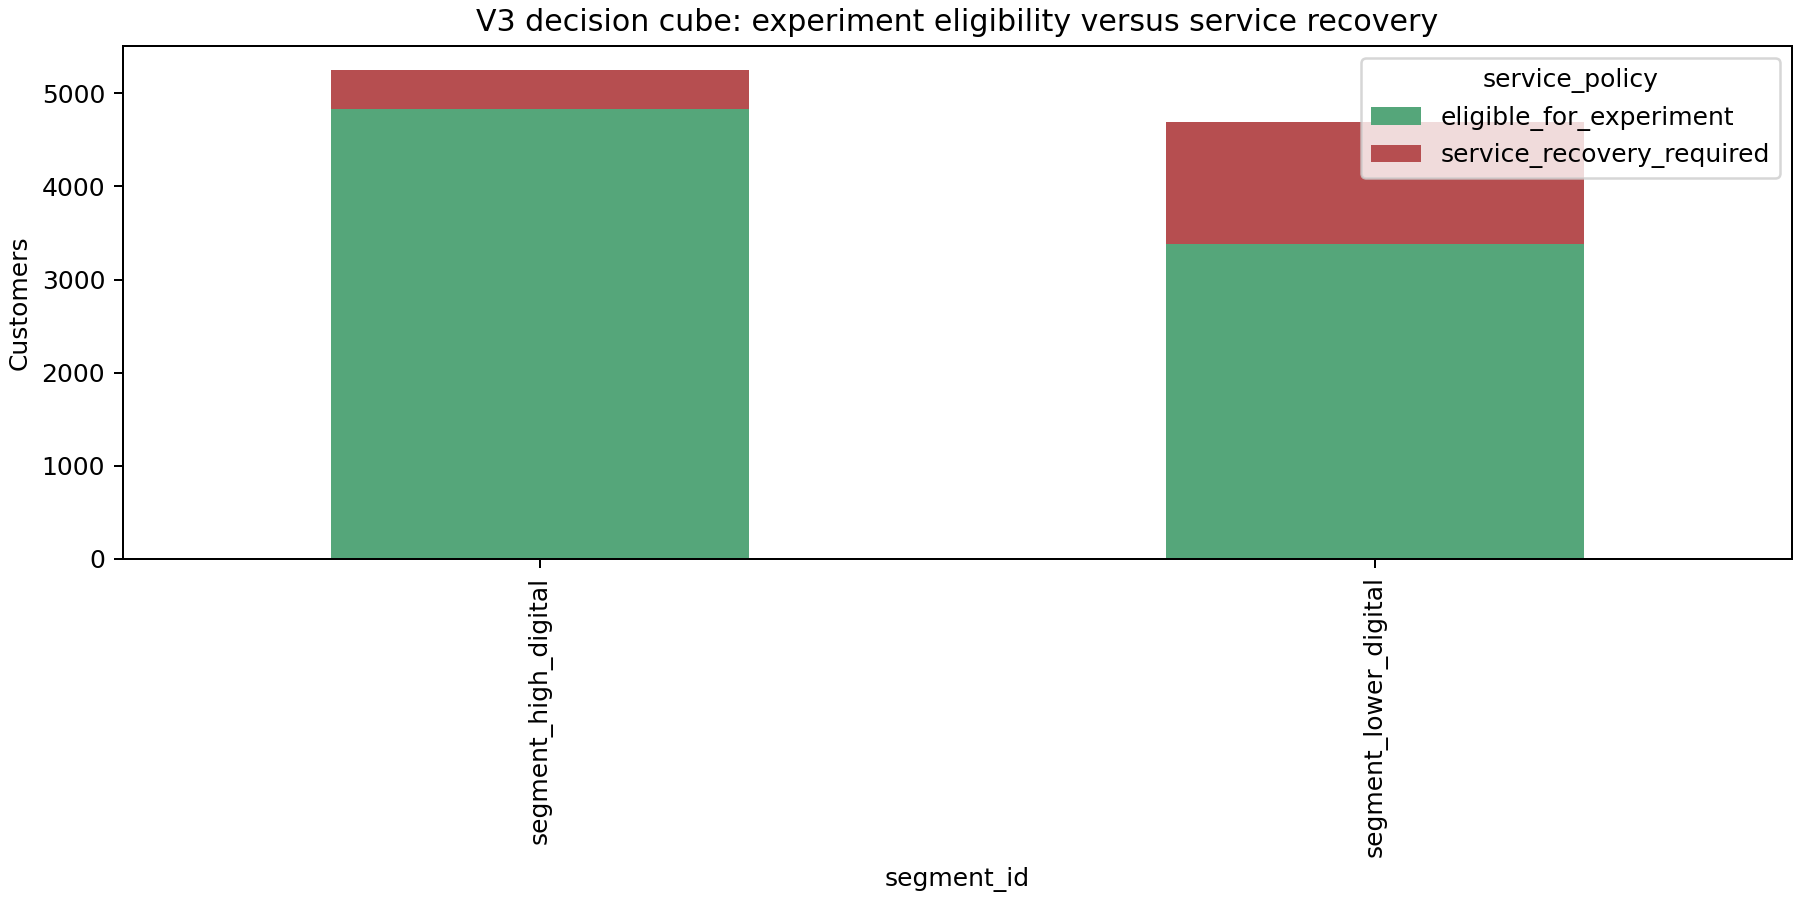
\includegraphics[width=0.82\textwidth]{figure/v3_decision_cube.png}
\caption{[\synthetic] V3 decision cube: simulated service-recovery routing versus a provisional experiment-routing state. It excludes real consent, contact-cap, suitability, contribution, and outcome data.}
\label{fig:cube}
\end{figure}

\subsection{Pilot operating playbook: exact journeys and control points}

The following playbook converts the two persona hypotheses into an executable, auditable pilot design. It is a \scenario{} and is not permission to contact any real person. Before randomization, CRM must freeze the eligibility list. A customer is eligible only if the intended channel is consented, the customer has not opted out, the contact cap has not been reached, there is no fraud or suitability hold, and no service case is open. Open cases route to Care and are excluded from marketing. Analytics then assigns eligible customers 50/50 within persona, stratified by recorded active-member flag and product count. Each customer ID may have one arm only; CRM records pilot ID, arm, randomisation seed, assignment time, suppression reason, and contact status. Manual arm switching is prohibited.

The generator places synthetic transaction dates roughly uniformly around days 14--15. This is a construction detail, not evidence of a payday or an optimal day-of-month contact strategy. The bank must instrument real timestamps before making timing claims.

\begin{longtable}{P{0.13\textwidth}P{0.16\textwidth}P{0.36\textwidth}P{0.16\textwidth}Y}
\caption{Detailed pilot journeys [\scenario]; all messages require consent and all contact stops on opt-out or case opening.}
\label{tab:pilot-journeys}\\
\toprule
\textbf{Pilot / arm} & \textbf{Timing} & \textbf{Action} & \textbf{Owner} & \textbf{Required control or log}\\
\midrule
\endfirsthead
\toprule
\textbf{Pilot / arm} & \textbf{Timing} & \textbf{Action} & \textbf{Owner} & \textbf{Required control or log}\\
\midrule
\endhead
\bottomrule
\endfoot
P1 Recovery & Day 0 & Review case, contact history, and consent; confirm route. & Care Operations & Routing confirmation within four working hours.\\
P1 Recovery & Day 1 & Contact through the consented channel; name the issue owner and next update. & Care agent & Log attempt, result, time, and channel.\\
P1 Recovery & Days 1--3 & Resolve or escalate according to case category and severity. & Operations & High severity escalates immediately; case has a daily status.\\
P1 Recovery & Days 3--7 & Confirm closure and ask whether the issue was resolved. & Care agent & Log closure, re-open, and satisfaction prompt.\\
P1 Recovery & Day 14 & Apply cooling period; only then re-check eligibility for another journey. & CRM & No promotion until closure is confirmed.\\
\midrule
P1 Coach & Day 0 & Select one simple task: view transactions, transfer money, or pay a bill. & Digital Product & Do not infer need or use balance/salary as a trigger.\\
P1 Coach & Day 1 & Deliver one in-app or consented-email instruction. & CRM & One message only; no cash incentive.\\
P1 Coach & Day 4 & Show contextual help only if the customer returns to the app. & Product & Do not follow the customer outside consent.\\
P1 Coach & Day 8 & Send one reminder if the task remains incomplete. & CRM & Suppress on opt-out or new open case.\\
P1 Coach & Day 14 & End the journey and log completion or drop-off. & Analytics & No further contact without a new, permitted trigger.\\
\midrule
P2 Concierge & Day 0 & Select one commonly used routine task: transfer, bill payment, or balance/card check. & Product & No targeting from gender, country, or balance.\\
P2 Concierge & Day 1 & On entry to the relevant task, show one shortcut and a clear processing status. & Product & Do not display a generic out-of-context pop-up.\\
P2 Concierge & Days 1--7 & When a task fails, show a repair path and connection to Care. & Product + Care & Do not force chat or call; log failure and escalation.\\
P2 Concierge & Day 7 & Send one help message only if consented and the task remains incomplete. & CRM & No cash offer or cross-sell.\\
P2 Concierge & Day 14 & Record completion, failed task, support contact, active days, and opt-out. & Analytics & Do not infer satisfaction from app use.\\
\midrule
P2 Value Review & Day 0 & Verify consent and the actual fee/benefit terms applicable to the customer. & CRM + Product & Never use simulated data as a reason for contact.\\
P2 Value Review & Day 1 & Send a concise summary of current products, fees/benefits, and a link to details. & CRM & Do not say that the customer is at risk of leaving.\\
P2 Value Review & Day 4 & Offer an explicit choice: learn more, request advice, or decline. & Customer & No default consent or pre-selected cross-sell.\\
P2 Value Review & Days 5--10 & Offer an appointment only to customers who request advice. & CRM / relationship manager & Do not sell an unsuitable product.\\
P2 Value Review & Day 14 & Record completion, voluntary request, opt-out, and complaint. & Analytics & Close the journey unless a permitted follow-up exists.\\
\end{longtable}

\subsection{KPI dictionary, guardrails, and decision rights}

Table~\ref{tab:pilot-kpis} provides the minimum operational scorecard. These are proposed measurement definitions, not results. Contact-cap, complaint, opt-out, and cost thresholds require written approval from CRM, Risk, and Finance before launch; no dashboard may display an unapproved threshold as an achieved business result.

\begin{table}[H]
\centering
\caption{Pilot KPI dictionary and cadence [\scenario].}
\label{tab:pilot-kpis}
\small
\begin{tabularx}{\textwidth}{P{0.24\textwidth}P{0.30\textwidth}P{0.15\textwidth}Y}
\toprule
\textbf{KPI} & \textbf{Formula / denominator} & \textbf{Owner and cadence} & \textbf{Decision use}\\
\midrule
Eligibility rate & Eligible customers / candidate customers in persona & CRM, weekly & Capacity and suppression audit.\\
Contact completion & Delivered contacts / assigned customers & CRM, weekly & Channel execution and missing-delivery review.\\
Case-closure SLA & Cases closed within SLA / opened cases & Care, weekly & Service-quality and routing decision.\\
Re-open rate & Re-opened cases / closed cases & Care, weekly & Whether closure was durable.\\
Journey completion & Completed target task / delivered journeys & Product, weekly & Leading indicator of usable assistance.\\
Opt-out rate & Opt-outs / delivered contacts & CRM, weekly & Pause guardrail.\\
Complaint rate & Complaints / contacted customers & Risk, weekly & Pause guardrail.\\
Incremental active-month rate & Treatment rate minus comparator rate & Analytics, days 30/60/90 & P1 experiment decision.\\
Incremental retention & Treatment retention minus comparator retention & Analytics, day 90 & P2 scale decision.\\
Cost per retained customer & Incremental cost / incremental retained customers & Finance, day 90 & Break-even and scale decision.\\
\bottomrule
\end{tabularx}
\end{table}

\begin{table}[H]
\centering
\caption{Pilot stop, pause, iterate, and scale rules [\scenario].}
\label{tab:pilot-gates}
\small
\begin{tabularx}{\textwidth}{P{0.18\textwidth}Y P{0.22\textwidth}}
\toprule
\textbf{Decision} & \textbf{Trigger} & \textbf{Required response}\\
\midrule
Stop immediately & Consent breach; suppressed customer contacted; open case routed to marketing; high-severity case has no owner; or critical data-quality failure. & Halt arm/contact, suppress customer where relevant, investigate, and notify Risk/Compliance.\\
Pause and review & Complaint, opt-out, or contact frequency exceeds approved guardrail; randomisation imbalance; or Care backlog exceeds SLA. & Pause enrolment within 24 hours; perform content, route, and data QA.\\
Iterate & Completion is low without a safety failure. & Product changes the journey; Analytics randomizes the revised version as a new treatment.\\
Scale & Lower 95\% CI of retention effect exceeds zero; guardrails are no worse than comparator; Finance approves cost per retained customer; Risk approves aggregate fairness review. & Executive sponsor approves controlled expansion with continued measurement.\\
\bottomrule
\end{tabularx}
\end{table}

\begin{table}[H]
\centering
\caption{Pilot RACI and weekly operating cadence [\scenario].}
\label{tab:pilot-raci}
\small
\begin{tabularx}{\textwidth}{P{0.30\textwidth}P{0.10\textwidth}P{0.10\textwidth}P{0.10\textwidth}P{0.10\textwidth}P{0.10\textwidth}Y}
\toprule
\textbf{Work} & \textbf{CRM} & \textbf{Care} & \textbf{Product} & \textbf{Finance} & \textbf{Risk} & \textbf{Analytics}\\
\midrule
Eligibility and randomisation & A/R & C & C & I & C & R\\
Service routing and SLA & I & A/R & C & I & C & I\\
Journey and content & R & C & A/R & I & C & C\\
Cost and break-even & I & I & C & A/R & I & C\\
Consent and guardrails & C & C & I & I & A/R & R\\
Experiment readout & I & I & C & C & C & A/R\\
\bottomrule
\end{tabularx}
\end{table}

Each Monday, Analytics reviews arm balance and data quality; Care reviews SLA, re-open, and backlog; CRM reviews delivery and opt-out; Product reviews completion and drop-off; Finance reviews spend; and Risk decides whether a pause is required. The executive sponsor receives a one-page weekly view of eligibility, contacts, consent failures, SLA, complaints, opt-outs, leading KPIs, spend, and data-quality alerts. At day 90, the decision is limited to stop, iterate, or scale.

\subsection{Artifact traceability and data still required}

Table~\ref{tab:persona-traceability} makes the customer-analysis chain auditable. The V3 persona documents supply the operating language and journey detail, while the counts and feature values in this report are reconciled to the current V3 CSV artifacts generated with seed 20261026. Earlier V2 and earlier V3 narrative drafts use different simulation releases and, where their counts conflict, are not combined with the current V3 results.

\begin{table}[H]
\centering
\caption{Traceability of the complete customer-analysis package.}
\label{tab:persona-traceability}
\small
\begin{tabularx}{\textwidth}{P{0.30\textwidth}P{0.24\textwidth}Y}
\toprule
\textbf{Source artifact} & \textbf{What is carried into this report} & \textbf{Evidence status and boundary}\\
\midrule
\texttt{manifest.json}, \texttt{assignments.csv}, \texttt{feature\_snapshot.csv} & Seed, 10,000-customer cohort, two segment sizes, and feature profiles. & \synthetic{}; reproducible simulation output.\\
\texttt{segment\_churn.csv}, static preprocessing manifest & Historical-label counts/rates, source audit, target separation, and Wilson intervals. & \observed{}; no prospective horizon.\\
\texttt{multi\_seed\_diagnostics.csv}, \texttt{distinctiveness.csv} & Five-seed ARI/share diagnostic, silhouette, and feature separation. & \synthetic{}; internal stability only.\\
Persona Atlas V3 and CEO Persona Playbook V3 Release & Linh/Minh dossiers, primary app tasks, treatment hypotheses, timing caveat, and power gate. & Mixed \synthetic{} + \observed{} + \scenario; names are not real customers.\\
Operating Playbook V3 & Eligibility freeze, four detailed journeys, KPI formulas, guardrails, RACI, and weekly cadence. & \scenario; no outreach or outcome has occurred.\\
\bottomrule
\end{tabularx}
\end{table}

Before the project can make a real customer insight or operational claim, the bank would need governed records for relationship-close reason, qualifying transaction and app events, case taxonomy and resolution, customer-stated need/satisfaction, channel consent and opt-out, campaign assignment and delivery, approved costs and contribution, and a genuine outcome window. Those inputs would replace the simulation; they are not optional detail to be filled with plausible assumptions.

\subsection{Customer-analysis conclusion}

The completed analysis supports one carefully bounded conclusion: the V3 simulation generates two large, stable behavioural patterns that are associated with materially different historical-label rates after clustering. This is enough to structure service hypotheses and a measurement plan. It is not enough to deploy a churn model, send a campaign, claim a return on investment, or assert that any pattern explains why customers leave. The highest-value next step is not another persona name; it is obtaining governed behavioural and outcome data, then testing whether the proposed treatments improve a real outcome relative to control.

\section{Churn prediction: required next module and current status}

\subsection{Target and status}

The intended target is the static historical \texttt{Exited}/\texttt{churn} label. The repository currently contains a deterministic demonstration classifier seam, not a trained classifier, calibrated probability, or evaluated champion. There are therefore no valid ROC-AUC, PR-AUC, precision, recall, lift, calibration, fairness, or threshold metrics to report. This section is a pre-specified implementation and reporting contract; it must not be mistaken for a completed model result.

\subsection{Required modelling protocol}

The completed module must compare a dummy baseline, Logistic Regression, Random Forest, and XGBoost. It must use a reproducible train/validation/untouched-test split, stratified where appropriate, with all imputation, encoding, scaling, feature selection, rebalancing, and calibration fit inside training folds only. A time split would be inappropriate until genuine longitudinal outcomes exist. The static target means the product must never present an output as an empirically validated next-quarter probability.

The evaluation pack must report prevalence, ROC-AUC, PR-AUC, precision, recall, F1, confusion matrix, Precision@K, Recall@K, Lift@K, top-decile capture, Brier score, calibration curve, threshold sensitivity, and subgroup results with a minimum cell-size rule. Threshold selection must start from a documented contact-capacity and scenario economics constraint, rather than the default 0.5. Synthetic-feature and source-only ablations are mandatory: an apparent score improvement from the generated extension would be evidence about this simulation, not about a real digital-bank signal.

\begin{table}[H]
\centering
\caption{Churn-prediction evidence ledger at report date [implementation status, not \modelestimate].}
\label{tab:churn-status}
\small
\begin{tabularx}{\textwidth}{P{0.29\textwidth}P{0.18\textwidth}Y}
\toprule
\textbf{Requirement} & \textbf{Status} & \textbf{Evidence needed before a claim}\\
\midrule
Static-label semantics & Complete & Source audit and visible no-horizon limitation.\\
Dummy/LR/RF/XGBoost comparison & BLOCKED & Versioned training code, split manifest, parameter budget, and reproduced table.\\
Untouched test and leakage suite & BLOCKED & Train-only transformations, negative leakage tests, and held-out metrics.\\
Calibration and operating threshold & BLOCKED & Validation-fitted calibrator, Brier/calibration plot, capacity and scenario assumptions.\\
Subgroup and error review & BLOCKED & Minimum-cell policy, aggregate fairness review, error cases, and OOD policy.\\
Online/offline parity & BLOCKED & Persisted preprocessing/model, contract test, versioned API response.\\
\bottomrule
\end{tabularx}
\end{table}

\section{Retention decision product, deployment, and MLOps design}

\subsection{Product scope}

The end product is a staff-facing Streamlit dashboard backed by a validated API, not a public customer-scoring tool. Its seven navigable views should be: Executive Cockpit; Portfolio Diagnostics; Segment Intelligence; Churn Risk Lab; Retention Strategy Lab; Operations/Staff Demo; and Monitoring \& Governance. Each display must state its denominator, population, data window, provenance tag, and limitation. Public demonstrations use only pseudonymous or synthetic examples. They do not expose raw customer-level exports, credentials, unapproved offers, or automatic contact actions.

The corresponding API contract should expose health and metadata endpoints plus validated prediction, segment-assignment, eligibility-decision, and aggregate-metrics endpoints. Each substantive response must carry a model/segment version, source status, and safe error message. Before a trained model exists, the system may expose demo wiring only when it is visibly labelled as such; it must not return a convincing-looking probability that users could mistake for a validated prediction.

\subsection{MLOps and monitoring requirements}

MLOps is the control loop around the model, not simply a deployment step. The release bundle must persist the same preprocessing, classifier, calibrator, segment centroids, feature schema, and policy version used offline. At run time, the system should log schema failures, nulls, input distribution drift, OOD distances, score-band distribution, cluster size and centroid distance, API latency/errors, policy violations, and model/version metadata. Calibration and realised performance can be monitored only after genuine delayed outcomes become available. Synthetic drift exercises are labelled \texttt{DEMO / SYNTHETIC}; they cannot demonstrate post-deployment accuracy.

Every alert needs a baseline, rationale, minimum sample size, owner, investigation step, challenger decision, and rollback condition. A drift threshold is a prompt for investigation, not permission to automatically retrain. Any retraining requires approved outcome data, a new leakage audit, comparative holdout evaluation, and a documented release decision.

\section{Business recommendations and implementation roadmap}

\subsection{Recommendation now}

Do not launch an incentive campaign or claim churn reduction from the present prototype. Instead, approve a controlled preparation phase. First, obtain a source licence record and real event definitions for qualifying transaction, app activity, service case, consent, contact cap, and relationship exit. Second, have Finance define contribution, costs, and a bounded break-even scenario. Third, have CRM and Risk approve suppressions and a pilot protocol. Only then should Analytics train the classification candidates and return with an evidence pack for a go/no-go decision.

The two segment-specific ideas are useful because they are operationally different. Customers with a lower simulated digital relationship should be considered for service-first routing and a simple reactivation experiment; customers with an established simulated digital routine should be protected from friction through contextual assistance or an opt-in value explanation. Neither group should receive a blanket incentive. This preserves the principle that a predicted label association is not a treatment recommendation.

\begin{table}[H]
\centering
\caption{30/60/90-day decision roadmap [\scenario].}
\label{tab:roadmap}
\small
\begin{tabularx}{\textwidth}{P{0.17\textwidth}P{0.25\textwidth}Y P{0.20\textwidth}}
\toprule
\textbf{Window} & \textbf{Primary owner} & \textbf{Deliverable and decision} & \textbf{No-go / stop condition}\\
\midrule
0--30 days & Data, CRM, Risk, Finance & Close source licence/provenance gap; define event grains, consent/contact rules, cost and contribution inputs; freeze pilot outcome and guardrails. & Licence/provenance unresolved; no consent policy; no usable outcome definition.\\
31--60 days & Analytics, Product, Care & Build audited event pipeline; complete EDA, leakage suite, clustering comparison, classifier candidates, calibration plan, and staff-demo contract tests. & Target leakage, unresolved data-quality failures, or no untouched test.\\
61--90 days & CRM, Analytics, Finance, Risk & Randomize only an eligible, adequately powered cohort; monitor delivery, complaint, opt-out, service SLA, and arm balance; report estimate with 95\% CI. & Consent breach, misrouted unresolved case, guardrail deterioration, or underpowered cohort.\\
Post-pilot & Executive sponsor & Stop, iterate, or scale based on incremental outcome, cost per saved customer, fairness exposure, and operational feasibility. & Lower CI does not clear approved threshold or harms exceed control.\\
\bottomrule
\end{tabularx}
\end{table}

\section{Limitations and conclusion}

This is a static-data and synthetic-behaviour prototype. Its strongest completed contribution is an auditable customer-analysis workflow that distinguishes observed source facts from simulation and from future experimentation. The historical churn label has no known prospective horizon. The behavioural tables, segment profiles, service cases, cash-flow scenarios, and decision cube are generated for design and testing; they do not describe a real bank's customers. The classification module is not yet trained, the economic inputs are not approved financial facts, and no treatment has been delivered or measured.

These boundaries do not make the work unhelpful. They make its next decision clear. The project now has a reproducible structure for moving from static labels to a governed retention system: validate source provenance, collect real event and outcome data, complete a leakage-safe model comparison, preserve the separation between segment, risk, value, and eligibility, and learn from a randomized pilot before scaling. Until those steps are complete, the correct project status is \textbf{IMPLEMENTATION IN PROGRESS / PROTOTYPE ONLY}, not production readiness.

\appendix
\section{Source Data Dictionary}
\label{app:data-dictionary}

Table~\ref{tab:source-data-dictionary} documents the static source fields used in the Bank X case. The churn label is held in a separate label table after preprocessing. The synthetic behavioural extension has its own field-level documentation in \texttt{docs/data\_dictionary\_v2.md}; it is not a source-data dictionary.

\begin{longtable}{P{0.22\textwidth}P{0.16\textwidth}P{0.34\textwidth}Y}
\caption{Static source data dictionary.}\label{tab:source-data-dictionary}\\
\toprule
\textbf{Field} & \textbf{Type} & \textbf{Business meaning} & \textbf{Analytical role}\\
\midrule
\endfirsthead
\toprule
\textbf{Field} & \textbf{Type} & \textbf{Business meaning} & \textbf{Analytical role}\\
\midrule
\endhead
\texttt{customer\_id} & string & Pseudonymous source customer identifier. & Primary key; excluded from modelling and segmentation.\\
\texttt{credit\_score} & integer & Source credit-score value. & Customer-profile attribute; candidate classifier input subject to governance.\\
\texttt{country} & category & Recorded geographic category: France, Germany, or Spain. & Portfolio comparison and aggregate fairness review; excluded from behavioural clustering and treatment selection.\\
\texttt{gender} & category & Recorded gender category. & Aggregate fairness review only; excluded from behavioural clustering and treatment selection.\\
\texttt{age} & integer & Customer age in years. & Customer-profile attribute; reviewed for fairness and modelling governance.\\
\texttt{tenure} & integer & Length of relationship in source years. & Customer-profile attribute and candidate classifier input.\\
\texttt{balance} & numeric & Recorded account balance in an unspecified source currency. & Profile attribute; not interpreted as revenue, contribution, or CLV.\\
\texttt{products\_number} & integer & Number of products held by the customer. & Relationship-depth attribute and candidate classifier input.\\
\texttt{credit\_card} & binary & Source indicator for credit-card ownership. & Product-holding attribute and candidate classifier input.\\
\texttt{active\_member} & binary & Source active-member flag. & Relationship-status attribute; not interpreted as app-session activity.\\
\texttt{estimated\_salary} & numeric & Source estimated-salary value in an unspecified currency. & Profile attribute; not interpreted as income paid into the bank, contribution, or CLV.\\
\texttt{churn} & binary & Static relationship-exit label, separated from the customer table during preprocessing. & Supervised-learning outcome and descriptive cross-tab only; never an input to segmentation or behaviour generation.\\
\texttt{source\_type} & string & Technical lineage marker for the Kaggle base. & Audit and provenance only.\\
\bottomrule
\end{longtable}

\bibliographystyle{apalike}
\bibliography{references}

\end{document}
